%%%%%%%%%%%%%%%%%%%%%%%%%%%%%%%%%%%%%%%%%%%%%%%%%%%%%%%%%%%%%%%%%%%%%%%%%%%%%%%%
%2345678901234567890123456789012345678901234567890123456789012345678901234567890
%        1         2         3         4         5         6         7         8
\documentclass[letterpaper, 10 pt, conference]{ieeeconf}  % Comment this line out
                                                          % if you need a4paper
%\documentclass[a4paper, 10pt, conference]{ieeeconf}      % Use this line for a4

\usepackage{float}
                                                          % paper
% uso paquete bookmark para tener bien los outlines.
\usepackage{bookmark}

% Configuro el idioma.
\usepackage[utf8]{inputenc} % Importante para mantener acentos.
\usepackage[spanish, activeacute]{babel} % Requiere: texlive-lang-spanish. Por primera vez hay que ejecutar: texconfig init> log

% Paquete para poder usar acentos en $$.
\usepackage{mathtools}
%\setmathfont{XITS math}

% Para los diagramas de flujo
\usepackage{tikz}
\usetikzlibrary{shapes.geometric, arrows}

% Elementos del diagrama
\tikzstyle{startstop} = [rectangle, rounded corners, 
minimum width=6em, 
minimum height=2em,
text centered, 
draw=black, 
fill=red!30]

\tikzstyle{io} = [trapezium, 
trapezium stretches=true, % A later addition
trapezium left angle=70, 
trapezium right angle=110, 
minimum width=6em, 
minimum height=2em, text centered, 
draw=black, fill=blue!30]

\tikzstyle{block} = [rectangle, 
minimum width=8em, 
minimum height=3em, 
text centered, 
text width=7.5em, 
draw=black, 
fill=white!30]

\tikzstyle{def} = [rectangle, 
minimum width=14em, 
minimum height=3em, 
text centered, 
text width=12em, 
draw=black, 
fill=purple!30]

\tikzstyle{swap_proccess} = [rectangle, 
minimum width=8em, 
minimum height=2em, 
text centered, 
text width=8em, 
draw=black, 
fill=orange!30]

\tikzstyle{process} = [rectangle, 
minimum width=6em, 
minimum height=2em, 
text centered, 
text width=6em, 
draw=black, 
fill=orange!30]

\tikzstyle{decision} = [diamond, 
minimum width=6em, 
minimum height=6em, 
text centered, 
draw=black, 
fill=green!30]
\tikzstyle{arrow} = [thick,->,>=stealth]

\usepackage{siunitx}

% package to get \url
\usepackage{hyperref}
\hypersetup{
  colorlinks=true,
  linkcolor=magenta,
  filecolor=magenta,
  citecolor=magenta,      
  urlcolor=magenta,
}

% Graficos electrónicos
\usepackage{circuitikz}

\IEEEoverridecommandlockouts                              % This command is only
                                                          % needed if you want to
                                                          % use the \thanks command
\overrideIEEEmargins
% See the \addtolength command later in the file to balance the column lengths
% on the last page of the document

\usepackage{graphicx}
\usepackage{graphics}

% styling for matlab/octave code.
\usepackage{matlab-prettifier}
% Configuracion, con esto puede agregar ñ.
\lstset{
  literate={ñ}{{\~n}}1
}

\usepackage{listings}

% The following packages can be found on http:\\www.ctan.org
%\usepackage{graphics} % for pdf, bitmapped graphics files
%\usepackage{epsfig} % for postscript graphics files
%\usepackage{mathptmx} % assumes new font selection scheme installed
%\usepackage{times} % assumes new font selection scheme installed
\usepackage{amsmath} % assumes amsmath package installed
%\usepackage{amssymb}  % assumes amsmath package installed

\title{\LARGE \bf Integrador TP N° 3}

\author{
  Tom\'as Vidal\\
  {\it Arquitectura de Computadoras}\\
  {\it Facultad de Ingenier\'ia, UNLP, La Plata, Argentina.}\\
  {\it 7 de Agosto, 2024.}
}                                            % <-this % stops a space


% comienzo

% INTRO


% Figura
\newcommand{\image}[2] {
  \begin{figure}[H]
    \centering
    \includegraphics[width=0.43\textwidth]{./#1.png}
    \caption{#2}
    \label{fig:#1}
  \end{figure}
}

% Codigo
% \begin{lstlisting}[style=Matlab-editor]
% % el código va aca
% dispc("HELLO WORLD");
% \end{lstlisting}

\begin{document}
\maketitle
\thispagestyle{empty}
\pagestyle{empty}

\section{Introducción}
El proyecto propuesto fue que, los alumnos involucrados en la programación del DuinoBot v2.3 hagan módulos por separados (librerías en C), y sean unificados en este proyecto. A continuación se explicita cómo se conectaron las diferentes librerías para poder controlar el robot, y la lógica de control general empleada.

\section{Librerías}
Todo el control del robot se basa en las siguientes librerías:
\begin{itemize}
  \item avr libc (librería estándar de AVR)
  \item avr-ir-necdecoder
  \item HotWheels
  \item theDistance
  \item IRDriver
  \item sensor-infrarojo
  \item UART
\end{itemize}

\subsection{avr libc}
Define puertos y aporta funcionalidades básicas para trabajar con los microcontroladores que tienen AVR.

\subsection{avr-ir-necdecoder}
Proporciona facilidad para conectar comandos por control IR (control remoto IR), con el protocolo NEC. En el proyecto se usa para pausar el robot y para salir del modo seguidor de línea.

\subsection{HotWheels}
Proporciona facilidad de control de los motores, lo hace enviando señales PWM a los puentes H de la placa. Se usa para hacer avanzar, frenar, rotar y retroceder el robot.

\subsection{theDistance}
Facilita el medir la distancia con el sensor ultrasónico (HC-SR04). Se usa para que no se choque cuando anda en modo libre.

\subsection{IRDriver}
Hace que sea facil la interacción con sensores IR, es una sub dependencia de NECdecoder y sensor-infrarojo

\subsection{sensor-infrarojo}
Proporciona facilidad con la interacción de los sensores de IR para seguir línea. Se emplea para detectar cuando se está pasando por una línea y, para seguirla.

\subsection{UART}
Es una sub dependencia de avr-ir-necdecoder. Se emplea para hacer testing.

\section{Lógica de control}
Se hizo que el robot avance hacia adelante, hasta que encuentre un obstáculo, entonces retrocede, gira unos 40 grados y luego continúa avanzando hacia adelante. En caso de encontrar una línea se activa el modo seguidor de línea y trata de seguirla; el modo seguidor de línea continua indefinidamente hasta que el usuario con un control remoto lo desactive. También se dispone la funcionalidad de que el usuario pueda pausar el robot por control remoto.

\section{Detalles de la placa y el robot}
El robot es el múltiplo N6, desarrollado por RobotGroup, con la versión de hardware DuinoBot v2.3 (ver \ref{fig:robot}). El microcontrolador que posee la placa (\ref{fig:placa}) ATMega1284P.

\begin{figure}[H]
  \centering
  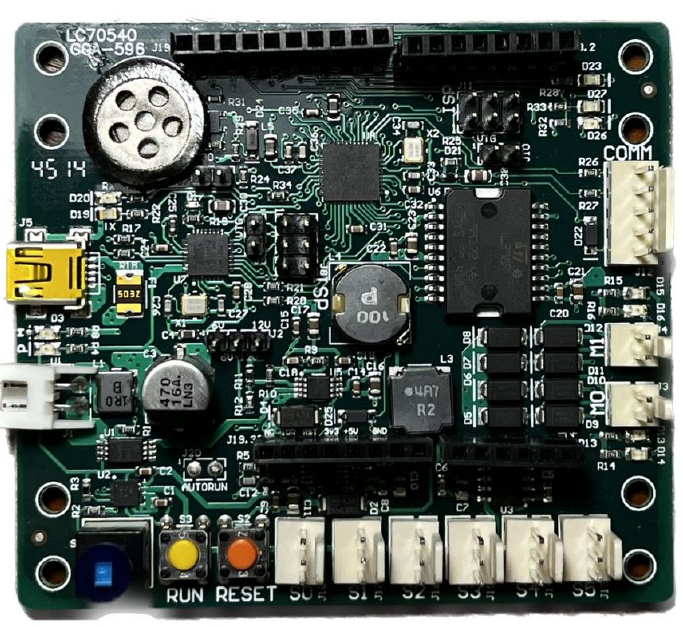
\includegraphics[width=0.43\textwidth]{./imagenes/placa.png}
  \caption{Placa DuinoBot v2.3}
  \label{fig:placa}
\end{figure}

\begin{figure}[H]
  \centering
  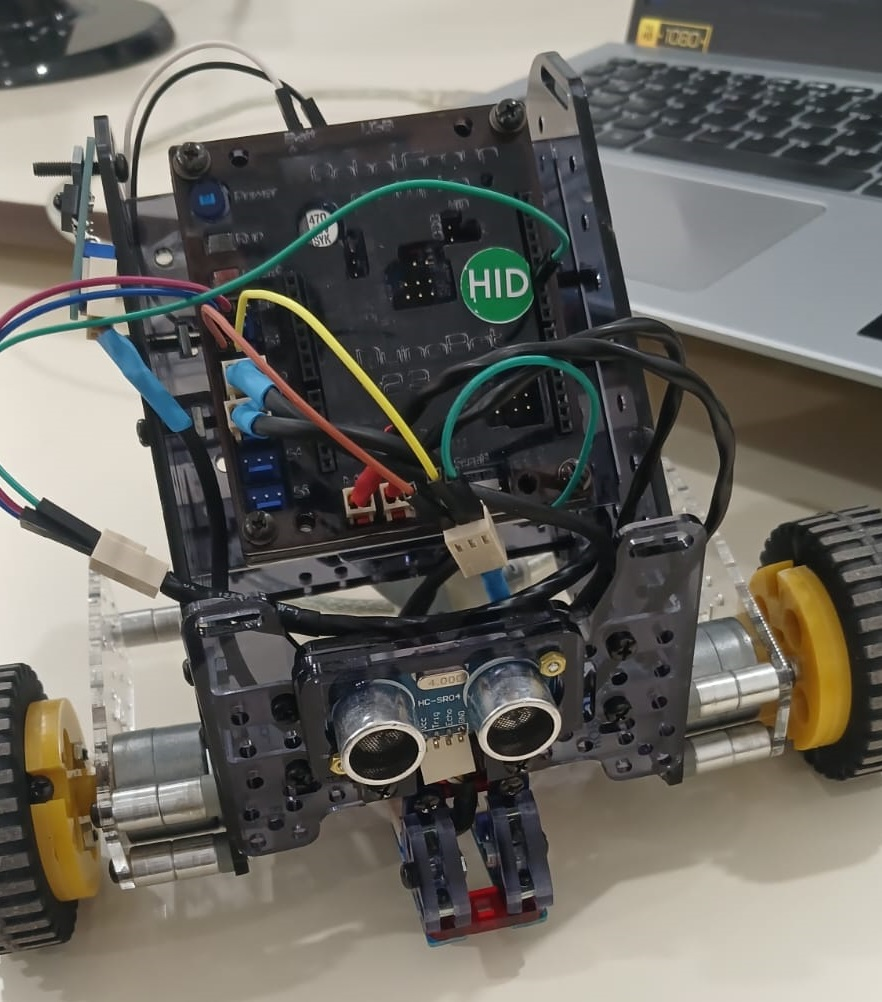
\includegraphics[width=0.43\textwidth]{./imagenes/robot.jpeg}
  \caption{Robot}
  \label{fig:robot}
\end{figure}

\section{Notas sobre el desarrollo}
El proyecto se encuentra publicado en \url{https://github.com/TomiVidal99/DuinoBot/}, y para que sea los más estándar, legible y mantenible, se optó por una estructura de archivos donde cada carpeta tiene un propósito concreto; además se hizo uso del programa ``make'' con un archivo de configuración ``Makefile'', para que se el compilado y flasheado del micro sea sensillo para el usuario.
Estructuas de archivos:
\begin{itemize}
  \item \textbf{lib}: dependencias externas (librerías que se emplearon, IRDriver, theDistance, etc.)
  \item \textbf{include}: los .h (defines.h)
  \item \textbf{src}: los .c (main.c)
  \item \textbf{Makefile}: archivo de configuración que especifica el compilado y flasheado
\end{itemize}

\end{document}
